% Created by tikzDevice version 0.12.3.1 on 2021-12-14 20:03:57
% !TEX encoding = UTF-8 Unicode
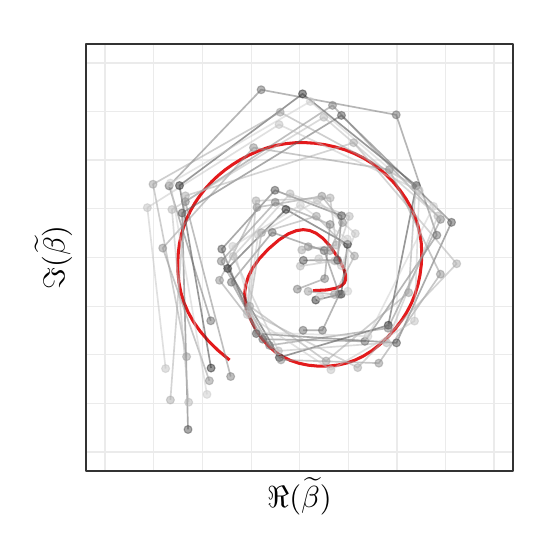
\begin{tikzpicture}[x=1pt,y=1pt]
\definecolor{fillColor}{RGB}{255,255,255}
\begin{scope}
\definecolor{drawColor}{RGB}{255,255,255}
\definecolor{fillColor}{RGB}{255,255,255}

\path[draw=drawColor,line width= 0.6pt,line join=round,line cap=round,fill=fillColor] (  0.00,  0.00) rectangle (180.67,180.68);
\end{scope}
\begin{scope}
\definecolor{fillColor}{RGB}{255,255,255}

\path[fill=fillColor] ( 20.71, 20.71) rectangle (175.17,175.17);
\definecolor{drawColor}{gray}{0.92}

\path[draw=drawColor,line width= 0.3pt,line join=round] ( 20.71, 45.29) --
	(175.17, 45.29);

\path[draw=drawColor,line width= 0.3pt,line join=round] ( 20.71, 80.39) --
	(175.17, 80.39);

\path[draw=drawColor,line width= 0.3pt,line join=round] ( 20.71,115.50) --
	(175.17,115.50);

\path[draw=drawColor,line width= 0.3pt,line join=round] ( 20.71,150.60) --
	(175.17,150.60);

\path[draw=drawColor,line width= 0.3pt,line join=round] ( 45.29, 20.71) --
	( 45.29,175.17);

\path[draw=drawColor,line width= 0.3pt,line join=round] ( 80.39, 20.71) --
	( 80.39,175.17);

\path[draw=drawColor,line width= 0.3pt,line join=round] (115.50, 20.71) --
	(115.50,175.17);

\path[draw=drawColor,line width= 0.3pt,line join=round] (150.60, 20.71) --
	(150.60,175.17);

\path[draw=drawColor,line width= 0.6pt,line join=round] ( 20.71, 27.74) --
	(175.17, 27.74);

\path[draw=drawColor,line width= 0.6pt,line join=round] ( 20.71, 62.84) --
	(175.17, 62.84);

\path[draw=drawColor,line width= 0.6pt,line join=round] ( 20.71, 97.94) --
	(175.17, 97.94);

\path[draw=drawColor,line width= 0.6pt,line join=round] ( 20.71,133.05) --
	(175.17,133.05);

\path[draw=drawColor,line width= 0.6pt,line join=round] ( 20.71,168.15) --
	(175.17,168.15);

\path[draw=drawColor,line width= 0.6pt,line join=round] ( 27.74, 20.71) --
	( 27.74,175.17);

\path[draw=drawColor,line width= 0.6pt,line join=round] ( 62.84, 20.71) --
	( 62.84,175.17);

\path[draw=drawColor,line width= 0.6pt,line join=round] ( 97.94, 20.71) --
	( 97.94,175.17);

\path[draw=drawColor,line width= 0.6pt,line join=round] (133.05, 20.71) --
	(133.05,175.17);

\path[draw=drawColor,line width= 0.6pt,line join=round] (168.15, 20.71) --
	(168.15,175.17);
\definecolor{drawColor}{RGB}{227,26,28}

\path[draw=drawColor,line width= 1.1pt,line join=round] (102.78, 85.96) --
	(107.80, 86.21) --
	(111.06, 86.85) --
	(113.03, 87.71) --
	(114.11, 88.72) --
	(114.61, 89.95) --
	(114.58, 91.65) --
	(113.82, 94.13) --
	(111.98, 97.68) --
	(109.10,101.89) --
	(106.39,104.85) --
	(103.92,106.70) --
	(101.58,107.70) --
	( 99.25,108.00) --
	( 96.75,107.63) --
	( 93.89,106.48) --
	( 90.52,104.31) --
	( 86.62,100.95) --
	( 83.38, 97.45) --
	( 81.04, 94.17) --
	( 79.45, 91.05) --
	( 78.50, 88.01) --
	( 78.13, 84.97) --
	( 78.32, 81.84) --
	( 79.10, 78.50) --
	( 80.57, 74.87) --
	( 82.49, 71.36) --
	( 84.55, 68.40) --
	( 86.77, 65.91) --
	( 89.15, 63.84) --
	( 91.73, 62.14) --
	( 94.55, 60.77) --
	( 97.67, 59.72) --
	(101.15, 59.01) --
	(104.90, 58.65) --
	(108.44, 58.68) --
	(111.78, 59.06) --
	(114.98, 59.80) --
	(118.06, 60.89) --
	(121.06, 62.35) --
	(124.03, 64.21) --
	(126.98, 66.53) --
	(129.92, 69.31) --
	(132.56, 72.24) --
	(134.82, 75.23) --
	(136.76, 78.29) --
	(138.38, 81.45) --
	(139.70, 84.73) --
	(140.74, 88.14) --
	(141.49, 91.73) --
	(141.96, 95.53) --
	(142.11, 99.33) --
	(141.94,102.92) --
	(141.46,106.36) --
	(140.68,109.66) --
	(139.59,112.85) --
	(138.18,115.98) --
	(136.44,119.05) --
	(134.34,122.10) --
	(131.91,125.06) --
	(129.36,127.71) --
	(126.69,130.05) --
	(123.89,132.12) --
	(120.94,133.92) --
	(117.83,135.47) --
	(114.52,136.78) --
	(110.98,137.85) --
	(107.22,138.68) --
	(103.51,139.21) --
	( 99.92,139.44) --
	( 96.45,139.40) --
	( 93.05,139.08) --
	( 89.71,138.49) --
	( 86.41,137.62) --
	( 83.12,136.46) --
	( 79.83,135.00) --
	( 76.66,133.32) --
	( 73.73,131.51) --
	( 71.02,129.59) --
	( 68.52,127.53) --
	( 66.20,125.34) --
	( 64.07,123.00) --
	( 62.09,120.50) --
	( 60.27,117.83) --
	( 58.63,115.01) --
	( 57.25,112.13) --
	( 56.11,109.18) --
	( 55.21,106.14) --
	( 54.55,102.99) --
	( 54.13, 99.72) --
	( 53.95, 96.29) --
	( 54.02, 92.68) --
	( 54.37, 88.90) --
	( 55.08, 85.20) --
	( 56.18, 81.63) --
	( 57.68, 78.14) --
	( 59.62, 74.70) --
	( 62.03, 71.27) --
	( 64.96, 67.83) --
	( 68.48, 64.37) --
	( 72.65, 60.87);
\definecolor{drawColor}{RGB}{51,51,51}

\path[draw=drawColor,draw opacity=0.50,line width= 0.6pt,line join=round] (103.79, 82.56) --
	(113.00, 84.70) --
	(115.28,102.70) --
	( 93.01,115.31) --
	( 71.97, 93.97) --
	( 90.67, 61.80) --
	(130.01, 73.46) --
	(140.12,123.90) --
	( 99.03,157.07) --
	( 54.56,123.92) --
	( 65.96, 57.99);
\definecolor{drawColor}{RGB}{87,87,87}

\path[draw=drawColor,draw opacity=0.50,line width= 0.6pt,line join=round] ( 99.32, 96.89) --
	(111.69, 96.99) --
	(113.13,113.04) --
	( 89.05,122.23) --
	( 69.84,100.99) --
	( 82.30, 70.44) --
	(132.98, 67.09) --
	(152.85,110.64) --
	(113.08,149.27) --
	( 55.51,114.01) --
	( 57.64, 35.79);
\definecolor{drawColor}{RGB}{110,110,110}

\path[draw=drawColor,draw opacity=0.50,line width= 0.6pt,line join=round] ( 99.21, 71.63) --
	(106.21, 71.64) --
	(112.32, 84.64) --
	(106.82,100.40) --
	( 88.07,107.00) --
	( 73.32, 89.00) --
	( 84.67, 68.41) --
	(121.55, 67.64) --
	(147.53,106.00) --
	(132.87,149.48) --
	( 84.06,158.55) --
	( 50.80,123.82) --
	( 65.85, 75.07);
\definecolor{drawColor}{RGB}{129,129,129}

\path[draw=drawColor,draw opacity=0.50,line width= 0.6pt,line join=round] ( 97.13, 86.49) --
	(107.03, 90.28) --
	(108.96,109.88) --
	( 89.16,117.89) --
	( 69.64, 96.61) --
	( 87.08, 66.19) --
	(129.90, 72.40) --
	(148.91,111.72) --
	(109.86,152.90) --
	( 56.68,118.11) --
	( 73.05, 54.92);
\definecolor{drawColor}{RGB}{145,145,145}

\path[draw=drawColor,draw opacity=0.50,line width= 0.6pt,line join=round] (101.06,101.82) --
	(108.93,100.42) --
	(113.48,110.56) --
	(106.00,120.08) --
	( 82.56,116.03) --
	( 69.04, 89.70) --
	( 91.24, 60.95) --
	(126.59, 59.76) --
	(148.83, 91.91) --
	(130.39,129.68) --
	( 81.31,137.63) --
	( 48.50,101.34) --
	( 65.35, 53.40);
\definecolor{drawColor}{RGB}{159,159,159}

\path[draw=drawColor,draw opacity=0.50,line width= 0.6pt,line join=round] (101.04, 85.70) --
	(110.55, 84.55) --
	(117.78, 98.47) --
	(104.01,112.84) --
	( 84.21,106.90) --
	( 79.92, 80.32) --
	(107.53, 60.53) --
	(137.37, 85.23) --
	(139.88,123.84) --
	( 90.94,150.44) --
	( 44.99,124.40) --
	( 57.11, 62.11);
\definecolor{drawColor}{RGB}{171,171,171}

\path[draw=drawColor,draw opacity=0.50,line width= 0.6pt,line join=round] ( 98.75,100.65) --
	(111.23,102.43) --
	(109.00,119.45) --
	( 82.21,118.42) --
	( 79.12, 78.59) --
	(118.96, 58.15) --
	(154.72, 95.68) --
	(117.50,139.42) --
	( 56.69,120.21) --
	( 51.27, 46.45);
\definecolor{drawColor}{RGB}{183,183,183}

\path[draw=drawColor,draw opacity=0.50,line width= 0.6pt,line join=round] ( 98.22, 94.84) --
	(110.66, 96.71) --
	(115.92,112.82) --
	( 94.51,120.95) --
	( 73.99, 98.36) --
	( 90.33, 64.16) --
	(129.43, 67.11) --
	(147.93,112.94) --
	(106.71,148.61) --
	( 51.82,115.26) --
	( 57.87, 45.63);
\definecolor{drawColor}{RGB}{194,194,194}

\path[draw=drawColor,draw opacity=0.50,line width= 0.6pt,line join=round] (104.89, 97.48) --
	(113.05, 95.00) --
	(118.08,106.57) --
	(104.36,118.60) --
	( 82.97,106.15) --
	( 79.05, 77.33) --
	(109.28, 57.37) --
	(139.48, 74.97) --
	(141.17,122.14) --
	( 90.53,145.98) --
	( 42.94,115.93) --
	( 49.54, 57.80);
\definecolor{drawColor}{RGB}{204,204,204}

\path[draw=drawColor,draw opacity=0.50,line width= 0.6pt,line join=round] (105.29, 83.82) --
	(115.37, 85.75) --
	(115.21,104.58) --
	( 98.24,116.90) --
	( 73.81,101.97) --
	( 82.84, 70.88) --
	(122.67, 69.48) --
	(146.36,116.41) --
	(101.83,154.30) --
	( 51.28,124.82) --
	( 64.49, 48.47);
\definecolor{drawColor}{RGB}{51,51,51}
\definecolor{fillColor}{RGB}{51,51,51}

\path[draw=drawColor,draw opacity=0.50,line width= 0.4pt,line join=round,line cap=round,fill=fillColor,fill opacity=0.50] (103.79, 82.56) circle (  1.43);

\path[draw=drawColor,draw opacity=0.50,line width= 0.4pt,line join=round,line cap=round,fill=fillColor,fill opacity=0.50] (113.00, 84.70) circle (  1.43);

\path[draw=drawColor,draw opacity=0.50,line width= 0.4pt,line join=round,line cap=round,fill=fillColor,fill opacity=0.50] (115.28,102.70) circle (  1.43);

\path[draw=drawColor,draw opacity=0.50,line width= 0.4pt,line join=round,line cap=round,fill=fillColor,fill opacity=0.50] ( 93.01,115.31) circle (  1.43);

\path[draw=drawColor,draw opacity=0.50,line width= 0.4pt,line join=round,line cap=round,fill=fillColor,fill opacity=0.50] ( 71.97, 93.97) circle (  1.43);

\path[draw=drawColor,draw opacity=0.50,line width= 0.4pt,line join=round,line cap=round,fill=fillColor,fill opacity=0.50] ( 90.67, 61.80) circle (  1.43);

\path[draw=drawColor,draw opacity=0.50,line width= 0.4pt,line join=round,line cap=round,fill=fillColor,fill opacity=0.50] (130.01, 73.46) circle (  1.43);

\path[draw=drawColor,draw opacity=0.50,line width= 0.4pt,line join=round,line cap=round,fill=fillColor,fill opacity=0.50] (140.12,123.90) circle (  1.43);

\path[draw=drawColor,draw opacity=0.50,line width= 0.4pt,line join=round,line cap=round,fill=fillColor,fill opacity=0.50] ( 99.03,157.07) circle (  1.43);

\path[draw=drawColor,draw opacity=0.50,line width= 0.4pt,line join=round,line cap=round,fill=fillColor,fill opacity=0.50] ( 54.56,123.92) circle (  1.43);

\path[draw=drawColor,draw opacity=0.50,line width= 0.4pt,line join=round,line cap=round,fill=fillColor,fill opacity=0.50] ( 65.96, 57.99) circle (  1.43);
\definecolor{drawColor}{RGB}{110,110,110}
\definecolor{fillColor}{RGB}{110,110,110}

\path[draw=drawColor,draw opacity=0.50,line width= 0.4pt,line join=round,line cap=round,fill=fillColor,fill opacity=0.50] ( 99.21, 71.63) circle (  1.43);

\path[draw=drawColor,draw opacity=0.50,line width= 0.4pt,line join=round,line cap=round,fill=fillColor,fill opacity=0.50] (106.21, 71.64) circle (  1.43);

\path[draw=drawColor,draw opacity=0.50,line width= 0.4pt,line join=round,line cap=round,fill=fillColor,fill opacity=0.50] (112.32, 84.64) circle (  1.43);

\path[draw=drawColor,draw opacity=0.50,line width= 0.4pt,line join=round,line cap=round,fill=fillColor,fill opacity=0.50] (106.82,100.40) circle (  1.43);

\path[draw=drawColor,draw opacity=0.50,line width= 0.4pt,line join=round,line cap=round,fill=fillColor,fill opacity=0.50] ( 88.07,107.00) circle (  1.43);

\path[draw=drawColor,draw opacity=0.50,line width= 0.4pt,line join=round,line cap=round,fill=fillColor,fill opacity=0.50] ( 73.32, 89.00) circle (  1.43);

\path[draw=drawColor,draw opacity=0.50,line width= 0.4pt,line join=round,line cap=round,fill=fillColor,fill opacity=0.50] ( 84.67, 68.41) circle (  1.43);

\path[draw=drawColor,draw opacity=0.50,line width= 0.4pt,line join=round,line cap=round,fill=fillColor,fill opacity=0.50] (121.55, 67.64) circle (  1.43);

\path[draw=drawColor,draw opacity=0.50,line width= 0.4pt,line join=round,line cap=round,fill=fillColor,fill opacity=0.50] (147.53,106.00) circle (  1.43);

\path[draw=drawColor,draw opacity=0.50,line width= 0.4pt,line join=round,line cap=round,fill=fillColor,fill opacity=0.50] (132.87,149.48) circle (  1.43);

\path[draw=drawColor,draw opacity=0.50,line width= 0.4pt,line join=round,line cap=round,fill=fillColor,fill opacity=0.50] ( 84.06,158.55) circle (  1.43);

\path[draw=drawColor,draw opacity=0.50,line width= 0.4pt,line join=round,line cap=round,fill=fillColor,fill opacity=0.50] ( 50.80,123.82) circle (  1.43);

\path[draw=drawColor,draw opacity=0.50,line width= 0.4pt,line join=round,line cap=round,fill=fillColor,fill opacity=0.50] ( 65.85, 75.07) circle (  1.43);
\definecolor{drawColor}{RGB}{129,129,129}
\definecolor{fillColor}{RGB}{129,129,129}

\path[draw=drawColor,draw opacity=0.50,line width= 0.4pt,line join=round,line cap=round,fill=fillColor,fill opacity=0.50] ( 97.13, 86.49) circle (  1.43);

\path[draw=drawColor,draw opacity=0.50,line width= 0.4pt,line join=round,line cap=round,fill=fillColor,fill opacity=0.50] (107.03, 90.28) circle (  1.43);

\path[draw=drawColor,draw opacity=0.50,line width= 0.4pt,line join=round,line cap=round,fill=fillColor,fill opacity=0.50] (108.96,109.88) circle (  1.43);

\path[draw=drawColor,draw opacity=0.50,line width= 0.4pt,line join=round,line cap=round,fill=fillColor,fill opacity=0.50] ( 89.16,117.89) circle (  1.43);

\path[draw=drawColor,draw opacity=0.50,line width= 0.4pt,line join=round,line cap=round,fill=fillColor,fill opacity=0.50] ( 69.64, 96.61) circle (  1.43);

\path[draw=drawColor,draw opacity=0.50,line width= 0.4pt,line join=round,line cap=round,fill=fillColor,fill opacity=0.50] ( 87.08, 66.19) circle (  1.43);

\path[draw=drawColor,draw opacity=0.50,line width= 0.4pt,line join=round,line cap=round,fill=fillColor,fill opacity=0.50] (129.90, 72.40) circle (  1.43);

\path[draw=drawColor,draw opacity=0.50,line width= 0.4pt,line join=round,line cap=round,fill=fillColor,fill opacity=0.50] (148.91,111.72) circle (  1.43);

\path[draw=drawColor,draw opacity=0.50,line width= 0.4pt,line join=round,line cap=round,fill=fillColor,fill opacity=0.50] (109.86,152.90) circle (  1.43);

\path[draw=drawColor,draw opacity=0.50,line width= 0.4pt,line join=round,line cap=round,fill=fillColor,fill opacity=0.50] ( 56.68,118.11) circle (  1.43);

\path[draw=drawColor,draw opacity=0.50,line width= 0.4pt,line join=round,line cap=round,fill=fillColor,fill opacity=0.50] ( 73.05, 54.92) circle (  1.43);
\definecolor{drawColor}{RGB}{145,145,145}
\definecolor{fillColor}{RGB}{145,145,145}

\path[draw=drawColor,draw opacity=0.50,line width= 0.4pt,line join=round,line cap=round,fill=fillColor,fill opacity=0.50] (101.06,101.82) circle (  1.43);

\path[draw=drawColor,draw opacity=0.50,line width= 0.4pt,line join=round,line cap=round,fill=fillColor,fill opacity=0.50] (108.93,100.42) circle (  1.43);

\path[draw=drawColor,draw opacity=0.50,line width= 0.4pt,line join=round,line cap=round,fill=fillColor,fill opacity=0.50] (113.48,110.56) circle (  1.43);

\path[draw=drawColor,draw opacity=0.50,line width= 0.4pt,line join=round,line cap=round,fill=fillColor,fill opacity=0.50] (106.00,120.08) circle (  1.43);

\path[draw=drawColor,draw opacity=0.50,line width= 0.4pt,line join=round,line cap=round,fill=fillColor,fill opacity=0.50] ( 82.56,116.03) circle (  1.43);

\path[draw=drawColor,draw opacity=0.50,line width= 0.4pt,line join=round,line cap=round,fill=fillColor,fill opacity=0.50] ( 69.04, 89.70) circle (  1.43);

\path[draw=drawColor,draw opacity=0.50,line width= 0.4pt,line join=round,line cap=round,fill=fillColor,fill opacity=0.50] ( 91.24, 60.95) circle (  1.43);

\path[draw=drawColor,draw opacity=0.50,line width= 0.4pt,line join=round,line cap=round,fill=fillColor,fill opacity=0.50] (126.59, 59.76) circle (  1.43);

\path[draw=drawColor,draw opacity=0.50,line width= 0.4pt,line join=round,line cap=round,fill=fillColor,fill opacity=0.50] (148.83, 91.91) circle (  1.43);

\path[draw=drawColor,draw opacity=0.50,line width= 0.4pt,line join=round,line cap=round,fill=fillColor,fill opacity=0.50] (130.39,129.68) circle (  1.43);

\path[draw=drawColor,draw opacity=0.50,line width= 0.4pt,line join=round,line cap=round,fill=fillColor,fill opacity=0.50] ( 81.31,137.63) circle (  1.43);

\path[draw=drawColor,draw opacity=0.50,line width= 0.4pt,line join=round,line cap=round,fill=fillColor,fill opacity=0.50] ( 48.50,101.34) circle (  1.43);

\path[draw=drawColor,draw opacity=0.50,line width= 0.4pt,line join=round,line cap=round,fill=fillColor,fill opacity=0.50] ( 65.35, 53.40) circle (  1.43);
\definecolor{drawColor}{RGB}{159,159,159}
\definecolor{fillColor}{RGB}{159,159,159}

\path[draw=drawColor,draw opacity=0.50,line width= 0.4pt,line join=round,line cap=round,fill=fillColor,fill opacity=0.50] (101.04, 85.70) circle (  1.43);

\path[draw=drawColor,draw opacity=0.50,line width= 0.4pt,line join=round,line cap=round,fill=fillColor,fill opacity=0.50] (110.55, 84.55) circle (  1.43);

\path[draw=drawColor,draw opacity=0.50,line width= 0.4pt,line join=round,line cap=round,fill=fillColor,fill opacity=0.50] (117.78, 98.47) circle (  1.43);

\path[draw=drawColor,draw opacity=0.50,line width= 0.4pt,line join=round,line cap=round,fill=fillColor,fill opacity=0.50] (104.01,112.84) circle (  1.43);

\path[draw=drawColor,draw opacity=0.50,line width= 0.4pt,line join=round,line cap=round,fill=fillColor,fill opacity=0.50] ( 84.21,106.90) circle (  1.43);

\path[draw=drawColor,draw opacity=0.50,line width= 0.4pt,line join=round,line cap=round,fill=fillColor,fill opacity=0.50] ( 79.92, 80.32) circle (  1.43);

\path[draw=drawColor,draw opacity=0.50,line width= 0.4pt,line join=round,line cap=round,fill=fillColor,fill opacity=0.50] (107.53, 60.53) circle (  1.43);

\path[draw=drawColor,draw opacity=0.50,line width= 0.4pt,line join=round,line cap=round,fill=fillColor,fill opacity=0.50] (137.37, 85.23) circle (  1.43);

\path[draw=drawColor,draw opacity=0.50,line width= 0.4pt,line join=round,line cap=round,fill=fillColor,fill opacity=0.50] (139.88,123.84) circle (  1.43);

\path[draw=drawColor,draw opacity=0.50,line width= 0.4pt,line join=round,line cap=round,fill=fillColor,fill opacity=0.50] ( 90.94,150.44) circle (  1.43);

\path[draw=drawColor,draw opacity=0.50,line width= 0.4pt,line join=round,line cap=round,fill=fillColor,fill opacity=0.50] ( 44.99,124.40) circle (  1.43);

\path[draw=drawColor,draw opacity=0.50,line width= 0.4pt,line join=round,line cap=round,fill=fillColor,fill opacity=0.50] ( 57.11, 62.11) circle (  1.43);
\definecolor{drawColor}{RGB}{171,171,171}
\definecolor{fillColor}{RGB}{171,171,171}

\path[draw=drawColor,draw opacity=0.50,line width= 0.4pt,line join=round,line cap=round,fill=fillColor,fill opacity=0.50] ( 98.75,100.65) circle (  1.43);

\path[draw=drawColor,draw opacity=0.50,line width= 0.4pt,line join=round,line cap=round,fill=fillColor,fill opacity=0.50] (111.23,102.43) circle (  1.43);

\path[draw=drawColor,draw opacity=0.50,line width= 0.4pt,line join=round,line cap=round,fill=fillColor,fill opacity=0.50] (109.00,119.45) circle (  1.43);

\path[draw=drawColor,draw opacity=0.50,line width= 0.4pt,line join=round,line cap=round,fill=fillColor,fill opacity=0.50] ( 82.21,118.42) circle (  1.43);

\path[draw=drawColor,draw opacity=0.50,line width= 0.4pt,line join=round,line cap=round,fill=fillColor,fill opacity=0.50] ( 79.12, 78.59) circle (  1.43);

\path[draw=drawColor,draw opacity=0.50,line width= 0.4pt,line join=round,line cap=round,fill=fillColor,fill opacity=0.50] (118.96, 58.15) circle (  1.43);

\path[draw=drawColor,draw opacity=0.50,line width= 0.4pt,line join=round,line cap=round,fill=fillColor,fill opacity=0.50] (154.72, 95.68) circle (  1.43);

\path[draw=drawColor,draw opacity=0.50,line width= 0.4pt,line join=round,line cap=round,fill=fillColor,fill opacity=0.50] (117.50,139.42) circle (  1.43);

\path[draw=drawColor,draw opacity=0.50,line width= 0.4pt,line join=round,line cap=round,fill=fillColor,fill opacity=0.50] ( 56.69,120.21) circle (  1.43);

\path[draw=drawColor,draw opacity=0.50,line width= 0.4pt,line join=round,line cap=round,fill=fillColor,fill opacity=0.50] ( 51.27, 46.45) circle (  1.43);
\definecolor{drawColor}{RGB}{183,183,183}
\definecolor{fillColor}{RGB}{183,183,183}

\path[draw=drawColor,draw opacity=0.50,line width= 0.4pt,line join=round,line cap=round,fill=fillColor,fill opacity=0.50] ( 98.22, 94.84) circle (  1.43);

\path[draw=drawColor,draw opacity=0.50,line width= 0.4pt,line join=round,line cap=round,fill=fillColor,fill opacity=0.50] (110.66, 96.71) circle (  1.43);

\path[draw=drawColor,draw opacity=0.50,line width= 0.4pt,line join=round,line cap=round,fill=fillColor,fill opacity=0.50] (115.92,112.82) circle (  1.43);

\path[draw=drawColor,draw opacity=0.50,line width= 0.4pt,line join=round,line cap=round,fill=fillColor,fill opacity=0.50] ( 94.51,120.95) circle (  1.43);

\path[draw=drawColor,draw opacity=0.50,line width= 0.4pt,line join=round,line cap=round,fill=fillColor,fill opacity=0.50] ( 73.99, 98.36) circle (  1.43);

\path[draw=drawColor,draw opacity=0.50,line width= 0.4pt,line join=round,line cap=round,fill=fillColor,fill opacity=0.50] ( 90.33, 64.16) circle (  1.43);

\path[draw=drawColor,draw opacity=0.50,line width= 0.4pt,line join=round,line cap=round,fill=fillColor,fill opacity=0.50] (129.43, 67.11) circle (  1.43);

\path[draw=drawColor,draw opacity=0.50,line width= 0.4pt,line join=round,line cap=round,fill=fillColor,fill opacity=0.50] (147.93,112.94) circle (  1.43);

\path[draw=drawColor,draw opacity=0.50,line width= 0.4pt,line join=round,line cap=round,fill=fillColor,fill opacity=0.50] (106.71,148.61) circle (  1.43);

\path[draw=drawColor,draw opacity=0.50,line width= 0.4pt,line join=round,line cap=round,fill=fillColor,fill opacity=0.50] ( 51.82,115.26) circle (  1.43);

\path[draw=drawColor,draw opacity=0.50,line width= 0.4pt,line join=round,line cap=round,fill=fillColor,fill opacity=0.50] ( 57.87, 45.63) circle (  1.43);
\definecolor{drawColor}{RGB}{194,194,194}
\definecolor{fillColor}{RGB}{194,194,194}

\path[draw=drawColor,draw opacity=0.50,line width= 0.4pt,line join=round,line cap=round,fill=fillColor,fill opacity=0.50] (104.89, 97.48) circle (  1.43);

\path[draw=drawColor,draw opacity=0.50,line width= 0.4pt,line join=round,line cap=round,fill=fillColor,fill opacity=0.50] (113.05, 95.00) circle (  1.43);

\path[draw=drawColor,draw opacity=0.50,line width= 0.4pt,line join=round,line cap=round,fill=fillColor,fill opacity=0.50] (118.08,106.57) circle (  1.43);

\path[draw=drawColor,draw opacity=0.50,line width= 0.4pt,line join=round,line cap=round,fill=fillColor,fill opacity=0.50] (104.36,118.60) circle (  1.43);

\path[draw=drawColor,draw opacity=0.50,line width= 0.4pt,line join=round,line cap=round,fill=fillColor,fill opacity=0.50] ( 82.97,106.15) circle (  1.43);

\path[draw=drawColor,draw opacity=0.50,line width= 0.4pt,line join=round,line cap=round,fill=fillColor,fill opacity=0.50] ( 79.05, 77.33) circle (  1.43);

\path[draw=drawColor,draw opacity=0.50,line width= 0.4pt,line join=round,line cap=round,fill=fillColor,fill opacity=0.50] (109.28, 57.37) circle (  1.43);

\path[draw=drawColor,draw opacity=0.50,line width= 0.4pt,line join=round,line cap=round,fill=fillColor,fill opacity=0.50] (139.48, 74.97) circle (  1.43);

\path[draw=drawColor,draw opacity=0.50,line width= 0.4pt,line join=round,line cap=round,fill=fillColor,fill opacity=0.50] (141.17,122.14) circle (  1.43);

\path[draw=drawColor,draw opacity=0.50,line width= 0.4pt,line join=round,line cap=round,fill=fillColor,fill opacity=0.50] ( 90.53,145.98) circle (  1.43);

\path[draw=drawColor,draw opacity=0.50,line width= 0.4pt,line join=round,line cap=round,fill=fillColor,fill opacity=0.50] ( 42.94,115.93) circle (  1.43);

\path[draw=drawColor,draw opacity=0.50,line width= 0.4pt,line join=round,line cap=round,fill=fillColor,fill opacity=0.50] ( 49.54, 57.80) circle (  1.43);
\definecolor{drawColor}{RGB}{204,204,204}
\definecolor{fillColor}{RGB}{204,204,204}

\path[draw=drawColor,draw opacity=0.50,line width= 0.4pt,line join=round,line cap=round,fill=fillColor,fill opacity=0.50] (105.29, 83.82) circle (  1.43);

\path[draw=drawColor,draw opacity=0.50,line width= 0.4pt,line join=round,line cap=round,fill=fillColor,fill opacity=0.50] (115.37, 85.75) circle (  1.43);

\path[draw=drawColor,draw opacity=0.50,line width= 0.4pt,line join=round,line cap=round,fill=fillColor,fill opacity=0.50] (115.21,104.58) circle (  1.43);

\path[draw=drawColor,draw opacity=0.50,line width= 0.4pt,line join=round,line cap=round,fill=fillColor,fill opacity=0.50] ( 98.24,116.90) circle (  1.43);

\path[draw=drawColor,draw opacity=0.50,line width= 0.4pt,line join=round,line cap=round,fill=fillColor,fill opacity=0.50] ( 73.81,101.97) circle (  1.43);

\path[draw=drawColor,draw opacity=0.50,line width= 0.4pt,line join=round,line cap=round,fill=fillColor,fill opacity=0.50] ( 82.84, 70.88) circle (  1.43);

\path[draw=drawColor,draw opacity=0.50,line width= 0.4pt,line join=round,line cap=round,fill=fillColor,fill opacity=0.50] (122.67, 69.48) circle (  1.43);

\path[draw=drawColor,draw opacity=0.50,line width= 0.4pt,line join=round,line cap=round,fill=fillColor,fill opacity=0.50] (146.36,116.41) circle (  1.43);

\path[draw=drawColor,draw opacity=0.50,line width= 0.4pt,line join=round,line cap=round,fill=fillColor,fill opacity=0.50] (101.83,154.30) circle (  1.43);

\path[draw=drawColor,draw opacity=0.50,line width= 0.4pt,line join=round,line cap=round,fill=fillColor,fill opacity=0.50] ( 51.28,124.82) circle (  1.43);

\path[draw=drawColor,draw opacity=0.50,line width= 0.4pt,line join=round,line cap=round,fill=fillColor,fill opacity=0.50] ( 64.49, 48.47) circle (  1.43);
\definecolor{drawColor}{RGB}{87,87,87}
\definecolor{fillColor}{RGB}{87,87,87}

\path[draw=drawColor,draw opacity=0.50,line width= 0.4pt,line join=round,line cap=round,fill=fillColor,fill opacity=0.50] ( 99.32, 96.89) circle (  1.43);

\path[draw=drawColor,draw opacity=0.50,line width= 0.4pt,line join=round,line cap=round,fill=fillColor,fill opacity=0.50] (111.69, 96.99) circle (  1.43);

\path[draw=drawColor,draw opacity=0.50,line width= 0.4pt,line join=round,line cap=round,fill=fillColor,fill opacity=0.50] (113.13,113.04) circle (  1.43);

\path[draw=drawColor,draw opacity=0.50,line width= 0.4pt,line join=round,line cap=round,fill=fillColor,fill opacity=0.50] ( 89.05,122.23) circle (  1.43);

\path[draw=drawColor,draw opacity=0.50,line width= 0.4pt,line join=round,line cap=round,fill=fillColor,fill opacity=0.50] ( 69.84,100.99) circle (  1.43);

\path[draw=drawColor,draw opacity=0.50,line width= 0.4pt,line join=round,line cap=round,fill=fillColor,fill opacity=0.50] ( 82.30, 70.44) circle (  1.43);

\path[draw=drawColor,draw opacity=0.50,line width= 0.4pt,line join=round,line cap=round,fill=fillColor,fill opacity=0.50] (132.98, 67.09) circle (  1.43);

\path[draw=drawColor,draw opacity=0.50,line width= 0.4pt,line join=round,line cap=round,fill=fillColor,fill opacity=0.50] (152.85,110.64) circle (  1.43);

\path[draw=drawColor,draw opacity=0.50,line width= 0.4pt,line join=round,line cap=round,fill=fillColor,fill opacity=0.50] (113.08,149.27) circle (  1.43);

\path[draw=drawColor,draw opacity=0.50,line width= 0.4pt,line join=round,line cap=round,fill=fillColor,fill opacity=0.50] ( 55.51,114.01) circle (  1.43);

\path[draw=drawColor,draw opacity=0.50,line width= 0.4pt,line join=round,line cap=round,fill=fillColor,fill opacity=0.50] ( 57.64, 35.79) circle (  1.43);
\definecolor{drawColor}{gray}{0.20}

\path[draw=drawColor,line width= 0.6pt,line join=round,line cap=round] ( 20.71, 20.71) rectangle (175.17,175.17);
\end{scope}
\begin{scope}
\definecolor{drawColor}{RGB}{0,0,0}

\node[text=drawColor,anchor=base,inner sep=0pt, outer sep=0pt, scale=  1.10] at ( 97.94,  7.64) {$\Re(\widetilde\beta)$};
\end{scope}
\begin{scope}
\definecolor{drawColor}{RGB}{0,0,0}

\node[text=drawColor,rotate= 90.00,anchor=base,inner sep=0pt, outer sep=0pt, scale=  1.10] at ( 13.08, 97.94) {$\Im(\widetilde\beta)$};
\end{scope}
\end{tikzpicture}
